\subsection{Năng lượng}
\begin{frame}
    \frametitle{Các bài toán quen thuộc}
    \begin{columns}
        \begin{column}{0.5\textwidth}
            \vspace{-14pt}

            \begin{figure}
                \centering
                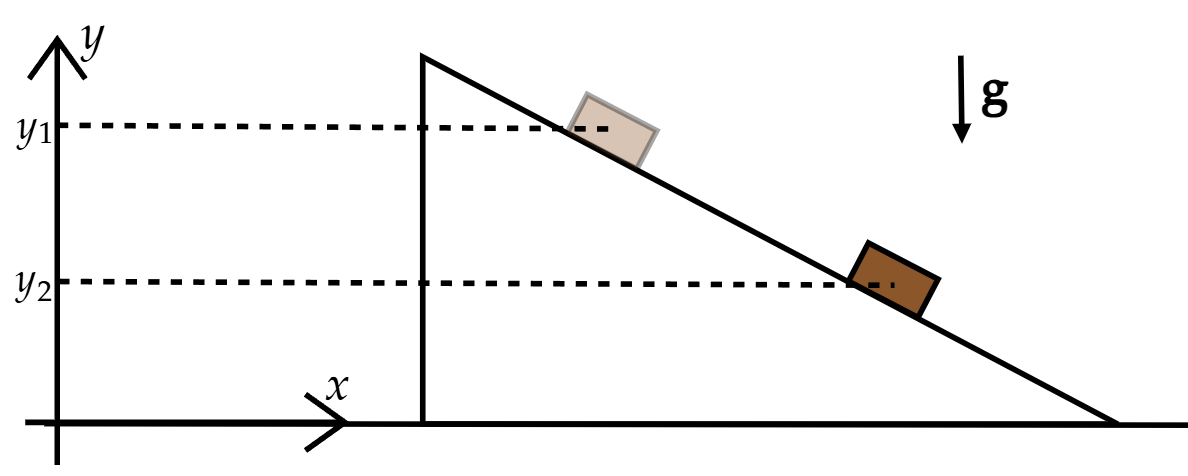
\includegraphics[width=7cm, height=3cm]{Content/Figure/gravity_energy.png}
            \end{figure}
            \[\frac{d}{dt}\left(\frac{mv^2}{2}-mgy\right)=0.\]
            \[\Delta\left(\frac{mv^2}{2}\right)-\int_{y_1}^{y_2}(-mg)dy=0.\]
        \end{column}
        \begin{column}{0.5\textwidth}
            \vspace{-14pt}

            \begin{figure}
                \centering
                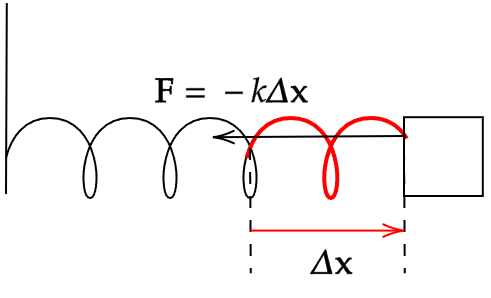
\includegraphics[width=5cm, height=3cm]{Content/Figure/springmass.png}
            \end{figure}
            \[\frac{d}{dt}\left(\frac{mv^2}{2}+\frac{k(\Delta x)^2}{2}\right)=0.\]
             \[\Delta\left(\frac{mv^2}{2}\right)-\int_{ x_1}^{x_2}(-k\Delta x)dx =0.\]
        \end{column}
    \end{columns}
\end{frame}
\begin{frame}
    \frametitle{Động năng, công, và thế năng}
    \begin{itemize}
        \item Đại lượng \(K=\frac{mv^2}{2}\) được gọi là động năng.
        \item Đại lượng \(A=\int_{q_1}^{q_2}F_q dq\) được gọi là công.
        \item Đại lượng \(V(q)=-\int_{\mathcal{O}}^{q}F_q(q)dq\) được gọi là thế năng.
    \end{itemize}
    Định lý biến thiên động năng: \[\frac{dK}{dt}=\sum \mathbf{F}\cdot\mathbf{v}.\]
    Nếu công của tất cả các lực tác dụng có thể được viết dưới dạng một hàm thế năng \(V(q)\), thì \emph{cơ năng} bảo toàn:
    \[E=K+V=const.\]
    \vspace{-16pt}

    Chú ý: Không phải công của mọi lực chỉ phụ thuộc vào toạ độ đều có thể viết dưới dạng thế năng.
\end{frame}
